%卒論概要テンプレート ver. 4.0

\documentclass[uplatex,twocolumn,dvipdfmx]{jsarticle}
\usepackage[top=22mm,bottom=22mm,left=22mm,right=22mm]{geometry}
\setlength{\columnsep}{11mm}
\usepackage[T1]{fontenc}
\usepackage{txfonts}
\usepackage[expert,deluxe]{otf}
\usepackage[dvipdfmx,hiresbb]{graphicx}
\usepackage[dvipdfmx]{hyperref}
\usepackage{pxjahyper}
\usepackage{secdot}





%タイトルと学生番号,名前だけ編集すること
\title{\vspace{-5mm}\fontsize{14pt}{0pt}\selectfont 文書自動添削システムによる学生の文書改善履歴の調査}
\author{\normalsize プロジェクトマネジメントコース 矢吹研究室 1442031 氏名 小山隆太郎}
\date{}
\pagestyle{empty}
\begin{document}
\fontsize{10.5pt}{\baselineskip}\selectfont
\maketitle





%以下が本文
\section{序論}
学生が行う研究では,研究だけではなく文書を作成する時間が長い.卒業論文は文量が多く,執筆形式も指摘される.大量の文書を人の目で添削を行うことには限界があり,かかる労力は大きい.また,自分以外が読んでもわかりやすい文書を書く必要があり,文が長いほど理解が難しくなってしまう場合や,「だから」,「それで」といった口語が混じり,文書の質が落ちてしまうことがある.

このような状況に RedPen\cite{a} を執筆環境に導入することで,文書の質が向上すると考えた.RedPenは技術文書をターゲットにした文書自動添削ツールである.継続的インテグレーションを活用し,常に添削ツールが動作している状態にすることで,文書添削にかかる労力を軽減できると考えた.

\section{目的}
RedPenは学校や会社等の組織のルールに対応できるように設定が柔軟に行える仕様になっているほか,添削ルールを新たに作成できる仕様になっている.研究向けの文書添削システムを確立し,文書の質の向上と,作成時間の短縮を図ることを目的とする.

\section{手法}
\begin{enumerate}
\item 文書チェックプログラムを作成する.
\item GitHubに文書をアップロードすると,文書チェックプログラムが自動で動作するようにし,添削結果を出力する. 
\item 添削結果を記録し,文中のミスが減るか推移を得る.
\end{enumerate}

\section{結果}
矢吹研究室に所属する3年生の課題文を添削を行った際の,エラー数の推移は図\ref{conf}のとおりである.各折れ線が文章1本のエラー数の推移を表している.エラー数が減った文書の修正は以下のように行われた.

\begin{enumerate}
\item 「の」,「が」等の接続詞の多用や,同一単語の複数回利用を抑えたことで,文長を短くした.「丁度」,「ちょうど」といった同じ言葉の表記を統一し,数値の全角表記を半角に修正した. 
\item 「これ」,「あれら」等の指示語の利用を抑えた文書.「感じる」,「思う」といった感嘆符の利用を避け,断定系に修正した文書は右下がりの推移を得た.
\end{enumerate}

\begin{figure}[htb]
\centering
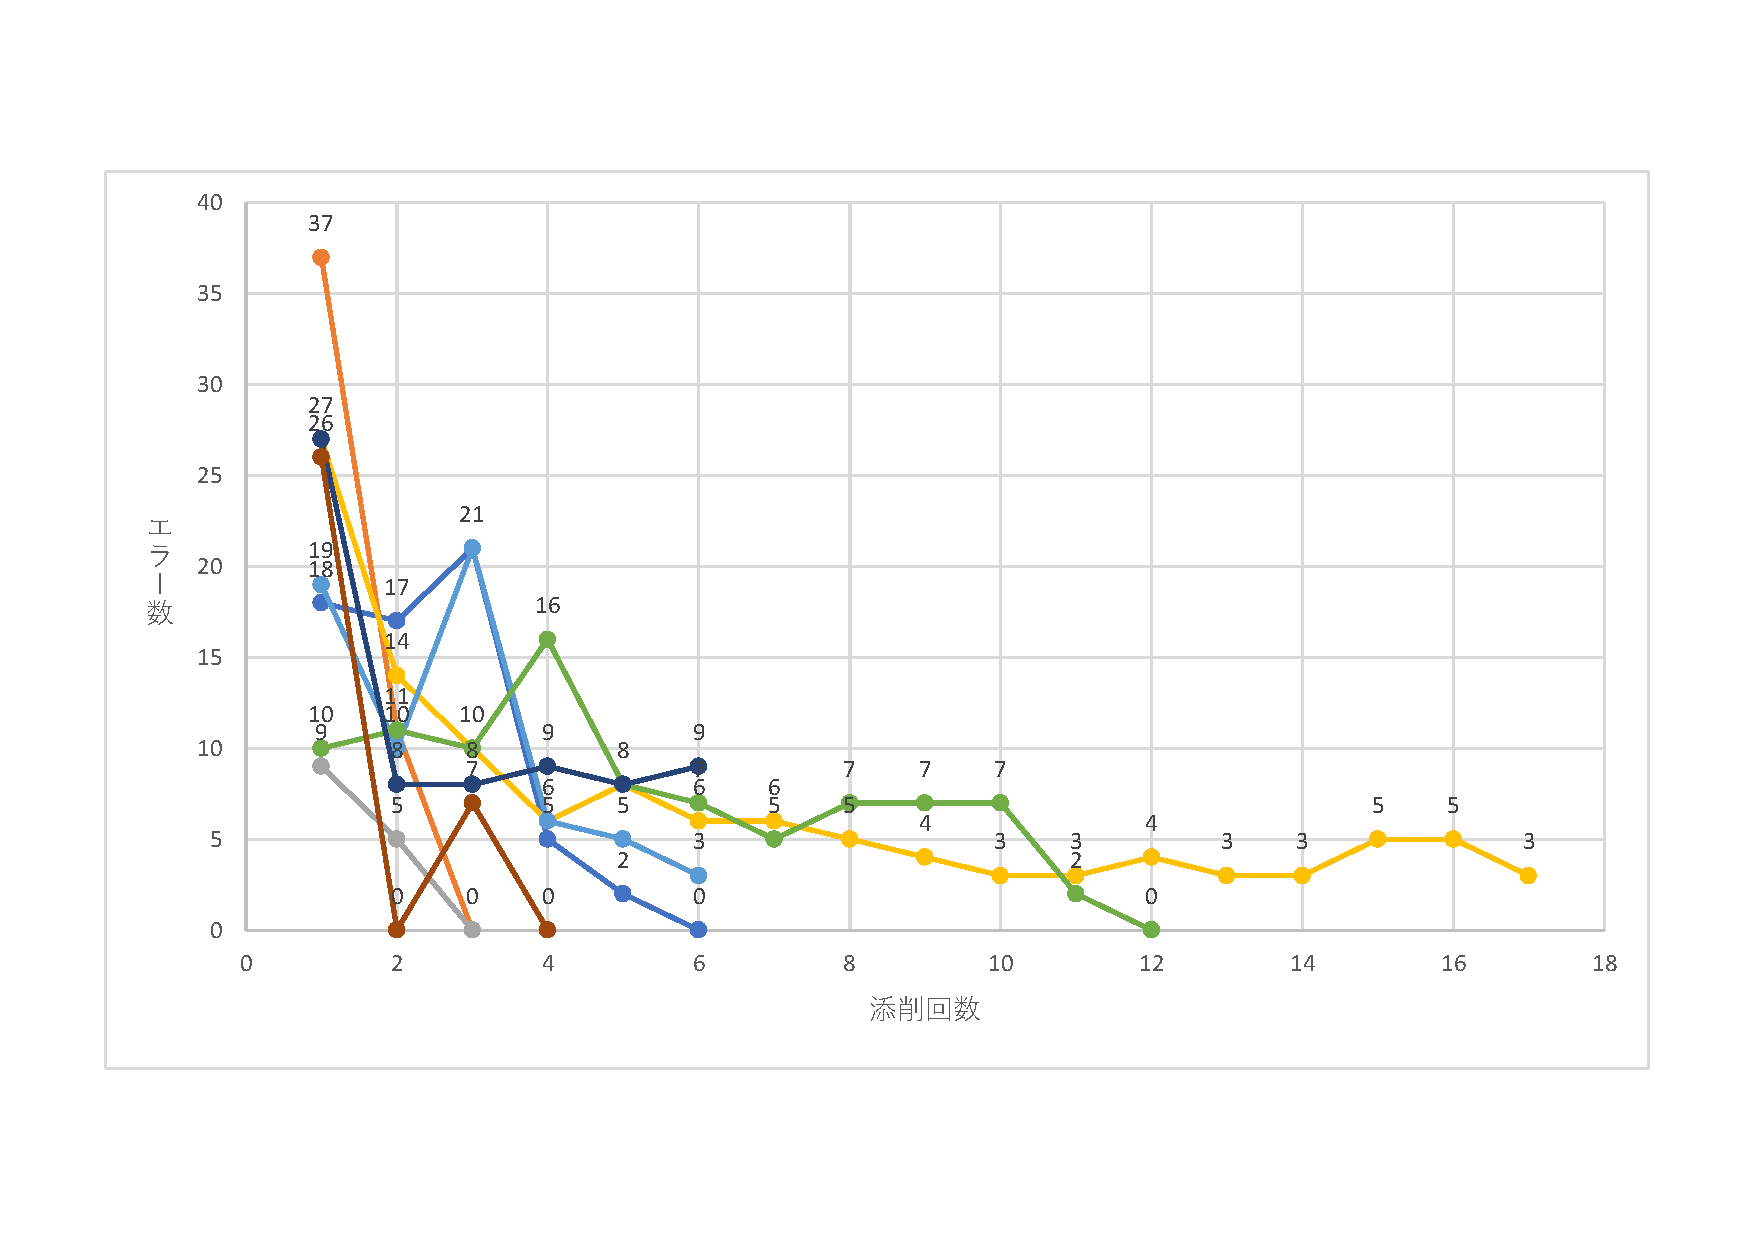
\includegraphics[width=6cm,clip]{redpen.pdf}
\caption{添削項数の推移}\label{conf}
\end{figure}

\section{考察}
専門知識を読み手にわかりやすく解説できるよ うに,指示語の利用を避けるルールと,断定系を使用するよう指示するルール等を作成したところ,指示語を使わず,専門用語を用いて解説する文書を多く見ることができた.また,曖昧な結論を書くことを抑えることで,読み手に安心感を与える文書を作成することができた.

\section{結論}
文書添削マシンの設定を考察し,執筆環境に実装することができた.添削マシンを利用することで,文書作成時間に変化があるのかを調べることができなかったため,検証が必要である.





\bibliographystyle{junsrt}
\bibliography{biblio}%「biblio.bib」というファイルが必要.

\end{document}
